\documentclass[french, 12pt]{article}

%-------------------------------------------------------------------------------
\usepackage[a4paper,top=2cm,bottom=2cm,left=2cm,right=2cm,marginparwidth=1.75cm]{geometry}
\usepackage{amsmath,amsfonts,amssymb,amsthm}
\usepackage[french]{babel}
\usepackage[utf8]{inputenc}
\usepackage[T1]{fontenc}
\usepackage{enumerate}
\usepackage{natbib}
\usepackage{graphicx}
\usepackage{xspace}
\usepackage{color,xcolor}
\usepackage{tikz}
\usepackage{remreset}
\usepackage{url}
% \usepackage{extsizes} % Permet \documentclass[french, 14pt]{extreport}
% \usepackage[a4paper,top=1cm,bottom=2cm,left=1cm,right=1cm,marginparwidth=.75cm]{geometry}
% \usepackage{minitoc}

\graphicspath{{../Figures/}}
% Environnement
\newtheorem{theorem}{Théorème}
\newtheorem{definition}{Définition}
\newtheorem{lemma}{Lemme}
\newtheorem{proposition}{Proposition}
\newtheorem*{theorem*}{Théorème}
\newtheorem*{definition*}{Définition}
\newtheorem*{proposition*}{Proposition}
\newtheorem*{corollary*}{Corollaire}
\newtheorem*{assumption*}{Hypothèse}
\newtheorem*{algorithm*}{Algorithme}
\newtheorem*{lemma*}{Lemme}
\newtheorem*{remark*}{Remarque}
\newtheorem*{exercise*}{Exercice}
\newtheorem{exercise}{Exercice}
\newcommand{\remark}{\bigskip\noindent\textbf{\textsl{Remarque.}}\xspace}
\newcommand{\remarks}{\bigskip\noindent\textbf{\textsl{Remarques.}}\xspace}
\newcommand{\parSR}[1]{\paragraph*{\textsl{#1}}\xspace}
\renewcommand{\proof}{\bigskip\noindent\underline{\textsl{Démonstration}.}\xspace}
\newcommand{\eproof}{$\blacksquare$}

% Effets, couleurs
\newcommand{\emphase}[1]{\textcolor{red}{#1}}
\newcommand{\demoProp}[1]{\noindent{\textbf{\textsl{Démonstration de la proposition \ref{#1} :}}}}
\newcommand{\itemdot}{\textbullet}

% Moments
\DeclareMathOperator{\Esp}{\mathbb{E}}
\DeclareMathOperator{\diag}{diag}
\DeclareMathOperator{\Cov}{\mathbb{C}ov}
\DeclareMathOperator{\tr}{tr}
\DeclareMathOperator{\Var}{\mathbb{V}}
\let\Pr\relax\DeclareMathOperator{\Pr}{\mathbb{P}}
\renewcommand{\d}{\text{d}}

% R, N, ...
\newcommand{\cst}{\text{cst}}
\newcommand{\Cbb}{\mathbb{C}}
\newcommand{\Ibb}{\mathbb{I}}
\newcommand{\Nbb}{\mathbb{N}}
\newcommand{\Rbb}{\mathbb{R}}
\newcommand{\Zbb}{\mathbb{Z}}

% Indicateurs

% Lois et ensembles
\newcommand{\Acal}{\mathcal{A}}
\newcommand{\Bcal}{\mathcal{B}}
\newcommand{\Ccal}{\mathcal{C}}
\newcommand{\Ecal}{\mathcal{E}}
\newcommand{\Gcal}{\mathcal{G}}
\newcommand{\Ical}{\mathcal{I}}
\newcommand{\Lcal}{\mathcal{L}}
\newcommand{\Mcal}{\mathcal{M}}
\newcommand{\Ncal}{\mathcal{N}}
\newcommand{\Pcal}{\mathcal{P}}
\newcommand{\Rcal}{\mathcal{R}}
\newcommand{\Scal}{\mathcal{S}}
\newcommand{\Ucal}{\mathcal{U}}
\newcommand{\Xcal}{\mathcal{X}}
\newcommand{\Ycal}{\mathcal{Y}}

% Comments
\newcommand{\SR}[2]{\textcolor{gray}{#1}\textcolor{red}{#2}}
\newcommand{\todo}[1]{\textcolor{red}{\`A faire~: {\sl #1}}}
\newcommand{\dessin}[1]{
\begin{center}\framebox{\begin{minipage}{\textwidth}
  \textcolor{purple}{#1}
\end{minipage}}\end{center}
\bigskip
}
\newcommand{\progres}[1]{
\begin{center}\framebox{\begin{minipage}{\textwidth}
  \textcolor{blue}{{\sl #1}}
\end{minipage}}\end{center}
\bigskip
}
\newcommand{\solution}[1]{
\begin{center}\framebox{\begin{minipage}{\textwidth}
  \noindent{\sl Solution :}
  #1
\end{minipage}}\end{center}
\bigskip
}
% \newcommand{\exemple}[1]{
% \begin{center}\framebox{\begin{minipage}{\textwidth}
%   \parSR{Exemple.}
%   #1
% \end{minipage}}\end{center}
% \bigskip
% }
\newcommand{\exemple}[1]{
\begin{breakbox}
  \parSR{Exemple.}
  #1
\end{breakbox}
\bigskip
}

\newcommand{\SRcorrect}[2]{\textcolor{gray}{#1}\textcolor{blue}{#2}}
\newcommand{\SRcomment}[1]{\textcolor{blue}{[{\sl SR: #1}]}}



% Section numbering
\usepackage{chngcntr}
% \renewcommand{\thepart}{\Roman{part}}
% \counterwithout{section}{part}
\setcounter{secnumdepth}{3}
\setcounter{tocdepth}{1}

% Proposition numbering
% \numberwithin{proposition}{section}
\numberwithin{exercise}{section}
\numberwithin{equation}{section}

%-------------------------------------------------------------------------------
%-------------------------------------------------------------------------------
\title{Note sur processus de Galton-Watson}
% \author{SR d'après \cite{Lam20} : Annexes}
% \date{\today}


%-------------------------------------------------------------------------------
%-------------------------------------------------------------------------------
\begin{document}
%-------------------------------------------------------------------------------
%-------------------------------------------------------------------------------


%-------------------------------------------------------------------------------
\section{Nombre de points fixes}
%-------------------------------------------------------------------------------
Il s'agit de montrer que la position de
$$
m = \Esp(X) = f'_X(1)
$$
par rapport à 1 contrôle la valeur de la parobabilité s'extinction $q$ dont on sait que c'est un point fixe de $f_X$ : 
$$
q = f_X(q).
$$

\bigskip
On écarte le cas $f_x(0) = 0 = \Pr\{X = 0\}$, qui implique que chaque individu a au moins un descendant et donc que $q = 0$.

\bigskip
La preuve repose sur l'étude des deux cas $\Pr\{X\geq 2\} = 0$ ou $\Pr\{X\geq 2\} > 0$. 

\begin{description}
  \item[Si $\Pr\{X\geq 2\} = 0$,] alors $X \in \{0, 1\}$, donc c'est une variable de Bernoulli $\Bcal(m)$ et $f_X(s)$ est linéaire, de pente $m \leq 1$. $f_X$ ne croise donc la première bissectrice qu'en $s = 1$.
  \item[Si $\Pr\{X\geq 2\} > 0$,] alors\footnote{L'étude de $f''_X(s)$ suggérée par l'un d'entre vous était donc plus que pertinente.}
  $$
  f''_X(s) = \Esp(X(X-1) s^X) = \sum_{x \geq 2} x (x-1) s^x > 0
  \qquad \text{pour } 0 < s \leq 1.
  $$
  La fonction $f_X$ est donc monotone croissante sur $[0, 1]$ et strictement convexe sur $(0, 1]$ avec $f_X(0) > 0$. Elle intersecte donc la première bissectrice dans $[0, 1]$, 
  \begin{itemize}
   \item seulement en $s=1$ si $m \leq 1$, 
   \item en $0 < s_1 < 1$ et $s_2=1$ si $m > 1$. 
  \end{itemize}
\end{description}

%-------------------------------------------------------------------------------
\section{Convergence vers le plus petit point fixe}
%-------------------------------------------------------------------------------

Pour montrer que $q$ est la plus petite solution de l'équation de point fixe $s = f_X(s)$, on note, pour $n \geq 0$:
$$
q_n := \Pr_1\{Z_n = 0\}.
$$
Par la proposition précédente on a:
$$
q_{n+1} = f_{Z_{n+1}}(0) = f_X \circ f_{Z_n} (0) = f_X(\Pr_1\{Z_n = 0\}) = f_X(q_n).
$$
La convergence vers le plus petit point fixe s'obtient en remarquant que, puisque $Z_0 = 1$, on a $q_0 = 0$ et en considérant la figure ci-dessous qui s'appuie sur le fait que $f_X(s) > s$ pour $s$ inférieur au plus petit point fixe.
$$
\begin{tabular}{cc}
  \begin{tabular}{lc}
    \textcolor{red}{\bf --} : $f_X(s)$ \\ ~ \\
    \textcolor{blue}{\bf--} : première bissectrice \\ ~ \\
    \textcolor{black}{\bf --} : itérations du point fixe
  \end{tabular}
  &
  \begin{tabular}{c}
  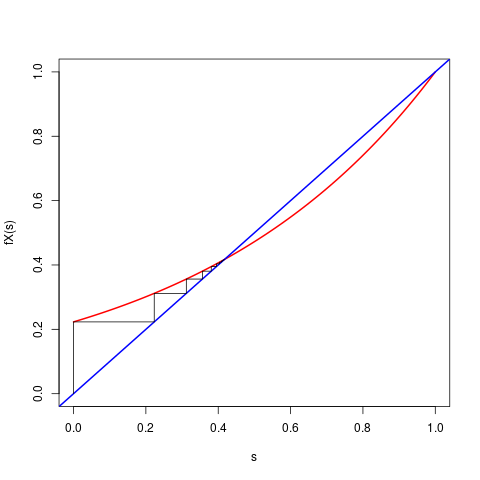
\includegraphics[width=.4\textwidth]{ExGaltonWatson-fixPoint}  
  \end{tabular}
\end{tabular}
$$

%-------------------------------------------------------------------------------
%-------------------------------------------------------------------------------
\end{document}
%-------------------------------------------------------------------------------
%-------------------------------------------------------------------------------


